\documentclass[11pt]{article}
\usepackage[hmargin=1in,vmargin=1in]{geometry}
\usepackage{xcolor}
\usepackage{amsmath,amssymb,amsfonts,url,sectsty,framed,tcolorbox,framed}
\usepackage{nicematrix}
\usepackage{algorithm2e}
\setcounter{MaxMatrixCols}{16}
\usepackage{tikz}
\usepackage{hyperref}
\usetikzlibrary{decorations.pathreplacing}
\newcommand{\pf}{{\bf Proof: }}
\newtheorem{theorem}{Theorem}
\newtheorem{lemma}{Lemma}
\newtheorem{proposition}{Proposition}
\newtheorem{definition}{Definition}
\newtheorem{remark}{Remark}
\newcommand{\qed}{\hfill \rule{2mm}{2mm}}


\begin{document}
%%%%%%%%%%%%%%%%%%%%%%%%%%%%%%%%%%%%%%%%%%%%%%%%%%%%%%%%%%%%%%%%%%%%%
\noindent
\rule{\textwidth}{1pt}
\begin{center}
{\bf [CS304] Introduction to Cryptography and Network Security}
\end{center}
Course Instructor: Dr. Dibyendu Roy \hfill Winter 2022-2023\\
Scribed by: Chitranshi Srivastava (202051055) \hfill Lecture 11 and 12 (Week 7)
\\
\rule{\textwidth}{1pt}
%%%%%%%%%%%%%%%%%%%%%%%%%%%%%%%%%%%%%%%%%%%%%%%%%%%%%%%%%%%
%write here

In previous week, we have studied the AES-128 algorithm. We discussed about the round function of AES - SubBytes, Shift Rows and Mix Column. We learnt about the Subbyte function in detail. In this week, we will study the rest of AES. After completing, AES, we will discuss Hash Functions in detail.

\section{Advanced Encryption Standard}
\subsection{Round Function of AES-128}
The Subbyte function was already discussed in the previous week.

\subsubsection{Shift Rows}
Shift Row function is a mapping from 128-bit to 128-bit. It takes a $4 \times 4$ matrix as input (the output of Subbyte function). It performs left circular shift on the elements of $i^{th}$ row by $i$ positions, where row index begins from 0.
\begin{center}
    Shift Rows: $\{0, 1\}^{128} \rightarrow \{0, 1\}^{128}$\\
    \vspace{1mm}
    $
    \begin{bmatrix}
        S_{00} & S_{01} & S_{02} & S_{03}\\
        S_{10} & S_{11} & S_{12} & S_{13}\\
        S_{20} & S_{21} & S_{22} & S_{23}\\
        S_{30} & S_{31} & S_{32} & S_{33}\\
    \end{bmatrix}
    \xrightarrow{Shift Rows}
    \begin{bmatrix}
        S_{00} & S_{01} & S_{02} & S_{03}\\
        S_{11} & S_{12} & S_{13} & S_{10}\\
        S_{22} & S_{23} & S_{20} & S_{21}\\
        S_{33} & S_{30} & S_{31} & S_{32}\\
    \end{bmatrix}
    $
\end{center}

\subsubsection{Mix Columns}
Mix columns, again, is a mapping from 128-bit to 128-bit. It also takes a $4 \times 4$ matrix as input (the output of Shift Rows function).
\begin{center}
    Mix Columns: $\{0, 1\}^{128} \rightarrow \{0, 1\}^{128}$\\
    \vspace{1mm}
    $(S_{ij})_{4 \times 4} \xrightarrow{Mix Columns} (S_{ij}^{'})_{4 \times 4}$
\end{center}
Consider the column $c \in {0,1,2,3}$ of matrix S.
\begin{center}
    column = $\begin{bmatrix}
        S_{0c}\\
        S_{1c}\\
        S_{2c}\\
        S_{3c}\\
    \end{bmatrix}$
\end{center}
The Mix Columns function is defined as follows. For i = 0 to i = 3, let $t_i$ be the polynomial constructed from $S_{ic}$. Define four polynomials as:
\begin{center}
    $u_0 = [(x * t_0) + (x + 1) * t_1 + t_2 + t_3]$ mod $(x^8 + x^4 + x^3 + x + 1)$\\
    \vspace{1mm}
    $u_1 = [t_0 + (x * t_1) + (x + 1) * t_2 + t_3]$ mod $(x^8 + x^4 + x^3 + x + 1)$\\
    \vspace{1mm}
    $u_2 = [t_0 + t_1 + (x * t_2) + (x + 1) * t_3]$ mod $(x^8 + x^4 + x^3 + x + 1)$\\
    \vspace{1mm}
    $u_3 = [(x + 1) * t_0 + t_1 + t_2 + (x * t_3)]$ mod $(x^8 + x^4 + x^3 + x + 1)$\\
\end{center}
Now, $S_{ij}^{'}$ is the binary 8-bits constructed using $u_i$. Therefore, 
\begin{center}
    $\begin{bmatrix}
        S_{0c}\\
        S_{1c}\\
        S_{2c}\\
        S_{3c}\\
    \end{bmatrix}
    \xrightarrow{Mix Columns}
    \begin{bmatrix}
        S_{0c}^{'}\\
        S_{1c}^{'}\\
        S_{2c}^{'}\\
        S_{3c}^{'}\\
    \end{bmatrix}$
\end{center}
Applying Mix Columns to each columns, will give us the entire $(S_{ij}^{'})_{4 \times 4}$ matrix. Therefore, Mix Column can be defined as a matrix multiplication as:
\begin{center}
    $
    (S_{ij}^{'})_{4 \times 4} = 
    \begin{bmatrix}
        x & x + 1 & 1 & 1\\
        1 & x & x+1 & 1\\
        1 & 1 & x & x+1\\
        x+1 & 1 & 1 & x\\
    \end{bmatrix}
    \times
    \begin{bmatrix}
        S_{00} & S_{01} & S_{02} & S_{03}\\
        S_{10} & S_{11} & S_{12} & S_{13}\\
        S_{20} & S_{21} & S_{22} & S_{23}\\
        S_{30} & S_{31} & S_{32} & S_{33}\\
    \end{bmatrix}
    $
    mod $(x^8 + x^4 + x^3 + x + 1)$
\end{center}
In terms of hexadecimal, the above multiplication can be represented as:
\begin{center}
    $
    (S_{ij}^{'})_{4 \times 4} = 
    \begin{bmatrix}
        2 & 3 & 1 & 1\\
        1 & 2 & 3 & 1\\
        1 & 1 & 2 & 3\\
        3 & 1 & 1 & 2\\
    \end{bmatrix}
    \times
    \begin{bmatrix}
        S_{00} & S_{01} & S_{02} & S_{03}\\
        S_{10} & S_{11} & S_{12} & S_{13}\\
        S_{20} & S_{21} & S_{22} & S_{23}\\
        S_{30} & S_{31} & S_{32} & S_{33}\\
    \end{bmatrix}
    $
    mod $(x^8 + x^4 + x^3 + x + 1)$
\end{center}

The polynomial $(x^8 + x^4 + x^3 + x + 1)$ is a primitive polynomial, hence, it is possible to construct the inverse of the Mix Columns function.\\
\newline
\textbf{Example:} Find $\begin{bmatrix}
        S_{00}^{'}\\
        S_{10}^{'}\\
        S_{20}^{'}\\
        S_{30}^{'}\\
    \end{bmatrix}$ after doing the Mix Column operation on $\begin{bmatrix}
        S_{0c}\\
        S_{1c}\\
        S_{2c}\\
        S_{3c}\\
    \end{bmatrix}$ where $S_{00} = 95, S_{10} = 65, S_{20} = fd, S_{30} = f3$.\\

\textbf{Solution:}
\begin{center}
    $S_{00} = 95 = 10010101 = x^7 + x^4 + x^2 + 1$\\
    $S_{10} = 65 = 01100101 = x^6 + x^5 + x^2 + 1$\\
    $S_{20} = fd = 11111101 = x^7 + x^6 + x^5 + x^4 + x^3 + x^2 + 1$\\
    $S_{30} = f3 = 11110011 = x^7 + x^6 + x^5 + x^4 + x + 1$\\
\end{center}
Now, let's calculate $S_{00}^{'}$.\\
\newline
$S_{00}^{'} = (x * S_{00} + (x+1) * S_{10} + S_{20} + S_{30})$ mod $(x^8 + x^4 + x^3 + x + 1)$\\
\newline
$S_{00}^{'} = ((x^8 + x^5 + x^3 + x) + (x^7 + x^5 + x^3 + x^2 + x + 1) + S_{20} + S_{30})$ mod $(x^8 + x^4 + x^3 + x + 1)$\\
\newline
$S_{00}^{'} = (x^8 + x^7 + x^3 + x + 1)$ mod $(x^8 + x^4 + x^3 + x + 1)$\\
\newline
$S_{00}^{'} = (x^7 + x^4) = 10010000 = (90)_{16}$\\
\newline
Similarly we can compute $S_{10}^{'}, S_{20}^{'}$ and $S_{30}^{'}$. Let's calculate each one of them.\\
\newline
    $S_{10}^{'} = (S_{00} + x * S_{10} + (x + 1) * S_{20} + S_{30})$ mod $(x^8 + x^4 + x^3 + x + 1)$\\
    \newline
    $S_{10}^{'} = (S_{00} + (x^7 + x^6 + x^3 + x) + (x^8 + x^2 + x + 1) + S_{30})$ mod $(x^8 + x^4 + x^3 + x + 1)$\\
    \newline
    $S_{10}^{'} = (x^8 + x^7 + x^5 + x^3 + x + 1)$ mod $(x^8 + x^4 + x^3 + x + 1)$\\
    \newline
    $S_{10}^{'} = (x^7 + x^5 + x^4) = 10110000 = (b0)_{16}$\\
\newline
Similarly, \\
\newline
    $S_{20}^{'} = (S_{00} + S_{10} + x * S_{20} + (x+1) * S_{30})$ mod $(x^8 + x^4 + x^3 + x + 1)$\\
    \newline
    $S_{20}^{'} = (S_{00} + S_{10} + (x^8 + x^7 + x^6 + x^5 + x^4 + x^3 + x) + (x^8 + x^4 + x^2 + 1))$ mod $(x^8 + x^4 + x^3 + x + 1)$\\
    \newline
    $S_{20}^{'} = (x^4 + x^3 + x^2 + x + 1)$ mod $(x^8 + x^4 + x^3 + x + 1)$\\
    \newline
    $S_{20}^{'} = (x^4 + x^3 + x^2 + x + 1) = 00011111 = (1f)_{16}$\\
    \newline
Similarly,\\
\newline
    $S_{30}^{'} = ((x+1) * S_{00} + S_{10} + S_{20} + x * S_{30})$ mod $(x^8 + x^4 + x^3 + x + 1)$\\
    \newline
    $S_{30}^{'} = ((x^8 + x^7 + x^5 + x^4 + x^3 + x^2 + x + 1) + S_{10} + S_{20} + (x^8 + x^7 + x^6 + x^5 + x^2 + x))$ mod $(x^8 + x^4 + x^3 + x + 1)$\\
    \newline
    $S_{30}^{'} = (x^7 + x^6 + 1)$ mod $(x^8 + x^4 + x^3 + x + 1)$\\
    \newline
    $S_{30}^{'} = (x^7 + x^6 + 1) = 11000001 = (c1)_{16}$\\
\newline
Therefore, we have,
\begin{center}
    $
    \begin{bmatrix}
        S_{00}^{'}\\
        S_{10}^{'}\\
        S_{20}^{'}\\
        S_{30}^{'}\\
    \end{bmatrix}
    =
    \begin{bmatrix}
        90\\
        b0\\
        1f\\
        c1\\
    \end{bmatrix}
    $
\end{center}

\subsection{Key Scheduling Algorithm of AES 128}
The key scheduling algorithm of AES-128 takes 128-bit key as input and generate 11 round keys of 128-bits each.
\begin{center}
    key = $(key[0], key[1],....., key[15])$ where each $key[i]$ is 1 byte long
\end{center}
We will generate 44 words (32-bit) - w[0], w[1],...., w[43]. We can see that (32 * 44)/128 = 11. Therefore, we can generate 11 round keys from these 44 words.\\

There are two functions involved in key scheduling algorithm. These are given below:
\begin{enumerate}
    \item ROTWORD($B_0B_1B_2B_3$): It takes a word as input and performs left circular shift of its bytes once (or left circular shift by 8 bits). Here, $B_0, B_1, B_2, B_3$ are bytes of the input word. The output of the ROTWORD function is:
    \begin{center}
        ROTWORD($B_0B_1B_2B_3$) = $B_1B_2B_3B_0$
    \end{center}

    \item SUBWORD($B_0B_1B_2B_3$): It takes a word as input and performs the Subbyte function (defined in round function of AES) of its bytes $B_0, B_1, B_2, B_3$. The output of SUBWORD function is:
    \begin{center}
        SUBWORD($B_0B_1B_2B_3$) = $B_0^{'} B_1^{'} B_2^{'} B_3^{'}$\\
        where $B_i^{'} = Subbytes(B_i)$ $\forall$ $i \in \{0,1,2,3\}$
    \end{center}
\end{enumerate}
Also, there are ten round constants (which are words, i.e, 32-bit) defined as:
\begin{center}
    $RCON[1] = 01000000$\\
    $RCON[2] = 02000000$\\
    $RCON[3] = 04000000$\\
    $RCON[4] = 08000000$\\
    $RCON[5] = 10000000$\\
    $RCON[6] = 20000000$\\
    $RCON[7] = 40000000$\\
    $RCON[8] = 80000000$\\
    $RCON[9] = 1b000000$\\
    $RCON[10] = 36000000$\\
\end{center}
Note that the values of constants written above are in hexadecimal. The 44 words are generated using the below algorithm.
\begin{center}
    \begin{algorithm}
        \For{$i \leftarrow 0$ to $3$}{
        $w_i \leftarrow key[4i] || key[4i+1] || key[4i+1] || key[4i+3]$;
        }
    
        \For{$i \leftarrow 4$ to $43$}{
            temp = w[i-1];\\
            \If{$i \% 4 == 0$}{
                temp = SUBWORD(ROTWORD(temp)) $\oplus$ RCON[i/4];
            }
            w[i] = w[i-1] $\oplus$ temp
        }
    \end{algorithm}
\end{center}

Now, the round keys will be given as:
\begin{center}
    $K_1 = w[0] || w[1] || w[2] || w[3]$\\
    \vspace{1mm}
    $K_2 = w[4] || w[5] || w[6] || w[7]$\\
    \vspace{1mm}
    .\\
    .\\
    $K_{11} = w[40] || w[41] || w[42] || w[43]$\\
    \vspace{1mm}
\end{center}

During decryption, we don't need the inverse of key scheduling algorithm as round keys are xored only. Hence, the same round keys will work during decryption.

\subsection{Inverse of Round Function}
As AES is based on Substitution Permutation Network (SPN) and for SPN we need inverse of round functions during decryption. Hence, we need inverse of round function for AES. The inverse of round function for round 1 to 9 is defined as:
\begin{center}
    $f_i^{-1} = Subbyte^{-1}(ShiftRows^{-1}(MixColumns^{-1}(S)))$ $\forall$ $i \in \{1,2,..,9\}$
\end{center}
For the $10^{th}$ round function, the inverse is defined as:
\begin{center}
    $f_{10}^{-1} = Subbyte^{-1}(ShiftRows^{-1}(S))$
\end{center}

\subsubsection{Inverse Subbyte Function}
During computation of Subbyte of a byte, say A, we took the 4 MSB bits as row number and 4 LSB bits as column number. Then, we looked up the value in the subbyte table. That is, 
\begin{center}
    $A = X || Y$\\
    \vspace{1mm}
    $Subbyte(A) = B = Subbyte\_Table[X][Y]$
\end{center}
Now, to compute inverse subbyte of B, we will find out the location of B in the table. Suppose, it is in row number $X'$ and column number $Y'$. Then,
\begin{center}
    $InverseSubbyte(B) = X' || Y'$
\end{center}

\subsubsection{Inverse Shift Row Function}
Inverse Shift Row function is defined as right circular shifting the elements of the $i_{th}$ row of the input matrix by $i$ positions. Note that $i \in \{0, 1, 2, 3\}$.
\begin{center}
    $
    \begin{bmatrix}
        S_{00} & S_{01} & S_{02} & S_{03}\\
        S_{10} & S_{11} & S_{12} & S_{13}\\
        S_{20} & S_{21} & S_{22} & S_{23}\\
        S_{30} & S_{31} & S_{32} & S_{33}\\
    \end{bmatrix}
    \xrightarrow{Inverse Shift Rows}
    \begin{bmatrix}
        S_{00} & S_{01} & S_{02} & S_{03}\\
        S_{13} & S_{10} & S_{11} & S_{12}\\
        S_{22} & S_{23} & S_{20} & S_{21}\\
        S_{31} & S_{32} & S_{33} & S_{30}\\
    \end{bmatrix}
    $
\end{center}

\subsubsection{Inverse Mix Column Function}
If we consider the Mix Column function as matrix multiplication (stated earlier), it can be written as:
\begin{center}
    $MixColumns(S) = S' = M * S$
\end{center}
It has been proven that,
\begin{center}
    $MixColumns(MixColumns(MixColumns(MixColumns(S)))) = I$\\
    \vspace{1mm}
    $M^4 * S = I$
\end{center}
where I is identity matrix. Therefore, inverse of M is $M^3$. Hence, 
\begin{center}
    $InverseMixColumns(S') = MixColumns(MixColumns(MixColumns(S'))) = S$
\end{center}

\subsection{Mode of Operation}
We know that we can encrypt 128 bit blocks using AES at once. Suppose we want to encrypt more data, let's say 256 bit data. We need some mechanism to encrypt this data. There are certain mode of operations which we will be discussing in encrypting more data than the block length. Few examples of mode of operation are mentioned below.
\begin{enumerate}
    \item Electronic CodeBook Mode (EBC)
    \item Cipher FeedBack Mode (CFB)
    \item Cipher Block Chaining Mode (CBC)
    \item Output FeedBack Mode (OFB)
    \item Counter Mode
    \item Count with Cipher Block Chaining Mode (CCM)
\end{enumerate}
We will be discussing the EBC and CBC mode in detail.\\

Let's say we have 256-bit of data that is to be encrypted using AES. We can first encrypt the first 128-bit block and then we can encrypt the second 128-bit block. Then, we can concatenate both the encrypted texts to get the ciphertext for the 256-bit data. Now, suppose there is an image of a human face (say of 200kB). We can follow the same approach that we discussed above to encrypt the image. However, there is a problem with this approach. There will be certain exactly identical parts in the image such as the right eye and the left eye. Let us consider the right eye is a 128-bit block and left eye is a 128-bit block. Since, these blocks are exactly similar, their corresponding ciphertext will also be exactly similar. Therefore, we can say that these two components of ciphertext, and hence plaintext, are same. That means, there is leakage of information. This mode of operation is known as Electronic CodeBook Mode (ECB). Therefore, in this mode we can get some patterns about plaintext from the ciphertext.

\subsubsection{Electronic CodeBook Mode}
As discussed above, in this mode, the plaintext is divided into continous blocks of l-bit size and each block is encrypted separately. The corresponding ciphertexts are concatenated in the same order to get the final ciphertext.
\begin{center}
    $M = m_0 || m_1 || ..... || m_t$ (plaintext)\\
    $len(m_i) = l-bit$ (each $m_i$ is a block, for AES, l = 128)
\end{center} 
\textbf{Encryption:}
\begin{center}
    $C = C_0 || C_1 || ..... || C_t$\\
    $C_i = Enc(m_i, K)$ $\forall$ $i \in \{0,1,...,t\}$
\end{center}
\textbf{Decryption:}
\begin{center}
    $M = m_0 || m_1 || ..... || m_t$\\
    $m_i = Dec(C_i, K)$ $\forall$ $i \in \{0,1,...,t\}$
\end{center}
The advantages of using ECB mode is that multiple blocks can be encrypted in parallel. However, it will reveal information if few blocks are same, i.e., if $m_i = m_j$ then $C_i = C_j$.

\subsubsection{Cipher Block Chaining Mode}
It is the most used mode of operation. It is used in applications like WhatsApp. There is a block of l-bit which is public. It is known as Initialization Vector (IV).\\
\newline
\textbf{Encryption:}
\begin{center}
    $M = m_1 || m_2 || ..... || m_t$ (plaintext)\\
    $len(m_i) = l-bit$ (each $m_i$ is a block, for AES, l = 128)\\
\end{center}
The encrypted text in CBC mode contains (n+1) blocks for a plaintext of n blocks. The ciphertext is computed as:
\begin{center}
    $C_0 = IV$\\
    $C_i = Enc(C_{i-1} \oplus m_i, K)$ $\forall$ $i \in \{1,2,3....,t\}$\\
    $C = C_0 || C_1 || ..... || C_t$
\end{center}

\begin{center}
    \tikzset{every picture/.style={line width=0.75pt}} 
    
    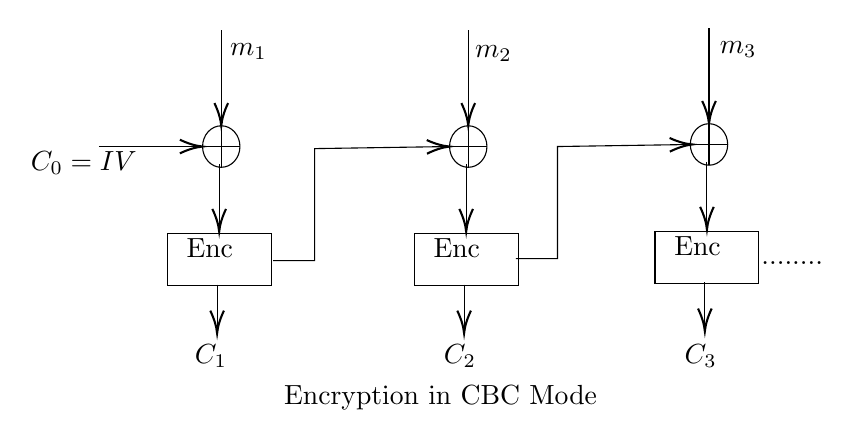
\begin{tikzpicture}[x=0.75pt,y=0.75pt,yscale=-1,xscale=1]
        \draw   (100,123) .. controls (100,117.48) and (104.03,113) .. (109,113) .. controls (113.97,113) and (118,117.48) .. (118,123) .. controls (118,128.52) and (113.97,133) .. (109,133) .. controls (104.03,133) and (100,128.52) .. (100,123) -- cycle ; \draw   (100,123) -- (118,123) ; \draw   (109,113) -- (109,133) ;
        \draw    (109,67) -- (109,111) ;
        \draw [shift={(109,113)}, rotate = 270] [color={rgb, 255:red, 0; green, 0; blue, 0 }  ][line width=0.75]    (10.93,-3.29) .. controls (6.95,-1.4) and (3.31,-0.3) .. (0,0) .. controls (3.31,0.3) and (6.95,1.4) .. (10.93,3.29)   ;
        \draw   (83,165) -- (133,165) -- (133,190) -- (83,190) -- cycle ; 
        \draw    (108,131.5) -- (108,162) ;
        \draw [shift={(108,164)}, rotate = 270] [color={rgb, 255:red, 0; green, 0; blue, 0 }  ][line width=0.75]    (10.93,-3.29) .. controls (6.95,-1.4) and (3.31,-0.3) .. (0,0) .. controls (3.31,0.3) and (6.95,1.4) .. (10.93,3.29)   ;
        \draw    (107,189.5) -- (107,211) ;
        \draw [shift={(107,213)}, rotate = 270] [color={rgb, 255:red, 0; green, 0; blue, 0 }  ][line width=0.75]    (10.93,-3.29) .. controls (6.95,-1.4) and (3.31,-0.3) .. (0,0) .. controls (3.31,0.3) and (6.95,1.4) .. (10.93,3.29)   ;
        \draw   (219,123) .. controls (219,117.48) and (223.03,113) .. (228,113) .. controls (232.97,113) and (237,117.48) .. (237,123) .. controls (237,128.52) and (232.97,133) .. (228,133) .. controls (223.03,133) and (219,128.52) .. (219,123) -- cycle ; \draw   (219,123) -- (237,123) ; \draw   (228,113) -- (228,133) ;
        \draw    (228,67) -- (228,111) ;
        \draw [shift={(228,113)}, rotate = 270] [color={rgb, 255:red, 0; green, 0; blue, 0 }  ][line width=0.75]    (10.93,-3.29) .. controls (6.95,-1.4) and (3.31,-0.3) .. (0,0) .. controls (3.31,0.3) and (6.95,1.4) .. (10.93,3.29)   ;
        \draw   (202,165) -- (252,165) -- (252,190) -- (202,190) -- cycle ;
        \draw    (227,131.5) -- (227,162) ;
        \draw [shift={(227,164)}, rotate = 270] [color={rgb, 255:red, 0; green, 0; blue, 0 }  ][line width=0.75]    (10.93,-3.29) .. controls (6.95,-1.4) and (3.31,-0.3) .. (0,0) .. controls (3.31,0.3) and (6.95,1.4) .. (10.93,3.29)   ; 
        \draw    (226,189.5) -- (226,211) ;
        \draw [shift={(226,213)}, rotate = 270] [color={rgb, 255:red, 0; green, 0; blue, 0 }  ][line width=0.75]    (10.93,-3.29) .. controls (6.95,-1.4) and (3.31,-0.3) .. (0,0) .. controls (3.31,0.3) and (6.95,1.4) .. (10.93,3.29)   ;
        \draw   (335,122) .. controls (335,116.48) and (339.03,112) .. (344,112) .. controls (348.97,112) and (353,116.48) .. (353,122) .. controls (353,127.52) and (348.97,132) .. (344,132) .. controls (339.03,132) and (335,127.52) .. (335,122) -- cycle ; \draw   (335,122) -- (353,122) ; \draw   (344,112) -- (344,132) ;
        \draw    (344,66) -- (344,110) ;
        \draw [shift={(344,112)}, rotate = 270] [color={rgb, 255:red, 0; green, 0; blue, 0 }  ][line width=0.75]    (10.93,-3.29) .. controls (6.95,-1.4) and (3.31,-0.3) .. (0,0) .. controls (3.31,0.3) and (6.95,1.4) .. (10.93,3.29)   ;
        \draw   (318,164) -- (368,164) -- (368,189) -- (318,189) -- cycle ;
        \draw    (343,130.5) -- (343,161) ;
        \draw [shift={(343,163)}, rotate = 270] [color={rgb, 255:red, 0; green, 0; blue, 0 }  ][line width=0.75]    (10.93,-3.29) .. controls (6.95,-1.4) and (3.31,-0.3) .. (0,0) .. controls (3.31,0.3) and (6.95,1.4) .. (10.93,3.29)   ;
        \draw    (342,188.5) -- (342,210) ;
        \draw [shift={(342,212)}, rotate = 270] [color={rgb, 255:red, 0; green, 0; blue, 0 }  ][line width=0.75]    (10.93,-3.29) .. controls (6.95,-1.4) and (3.31,-0.3) .. (0,0) .. controls (3.31,0.3) and (6.95,1.4) .. (10.93,3.29)   ;
        \draw    (134,178) -- (154,178) -- (154,124) -- (217,123.03) ;
        \draw [shift={(219,123)}, rotate = 179.12] [color={rgb, 255:red, 0; green, 0; blue, 0 }  ][line width=0.75]    (10.93,-3.29) .. controls (6.95,-1.4) and (3.31,-0.3) .. (0,0) .. controls (3.31,0.3) and (6.95,1.4) .. (10.93,3.29)   ;
        \draw    (251,177) -- (271,177) -- (271,123) -- (334,122.03) ;
        \draw [shift={(336,122)}, rotate = 179.12] [color={rgb, 255:red, 0; green, 0; blue, 0 }  ][line width=0.75]    (10.93,-3.29) .. controls (6.95,-1.4) and (3.31,-0.3) .. (0,0) .. controls (3.31,0.3) and (6.95,1.4) .. (10.93,3.29)   ; 
        \draw    (50,123) -- (98,123) ;
        \draw [shift={(100,123)}, rotate = 180] [color={rgb, 255:red, 0; green, 0; blue, 0 }  ][line width=0.75]    (10.93,-3.29) .. controls (6.95,-1.4) and (3.31,-0.3) .. (0,0) .. controls (3.31,0.3) and (6.95,1.4) .. (10.93,3.29)   ;
        
        \draw (91,166) node [anchor=north west][inner sep=0.75pt]   [align=left] {Enc};
        \draw (95,217) node [anchor=north west][inner sep=0.75pt]   [align=left] {$C_1$};
        \draw (210,166) node [anchor=north west][inner sep=0.75pt]   [align=left] {Enc};
        \draw (215,217) node [anchor=north west][inner sep=0.75pt]   [align=left] {$C_2$};
        \draw (326,165) node [anchor=north west][inner sep=0.75pt]   [align=left] {Enc};
        \draw (331,217) node [anchor=north west][inner sep=0.75pt]   [align=left] {$C_3$};
        \draw (368,177) node [anchor=north west][inner sep=0.75pt]   [align=left] {........};
        \draw (16,124) node [anchor=north west][inner sep=0.75pt]   [align=left] {$C_0 = IV$};
        \draw (112,72) node [anchor=north west][inner sep=0.75pt]   [align=left] {$m_1$};
        \draw (230,73) node [anchor=north west][inner sep=0.75pt]   [align=left] {$m_2$};
        \draw (348,71) node [anchor=north west][inner sep=0.75pt]   [align=left] {$m_3$};
        \draw (138,237) node [anchor=north west][inner sep=0.75pt]   [align=left] {Encryption in CBC Mode};
    \end{tikzpicture}
\end{center}

\textbf{Decryption:}
\begin{center}
    $m_i = Dec(C_i, K) \oplus C_{i-1}$ $\forall$ $i \in \{1,2...,t\}$\\
    where $C_0 = IV$\\
    $M = m_1 || m_2 || ..... || m_t$
\end{center}

\begin{center}
    \tikzset{every picture/.style={line width=0.75pt}}      

    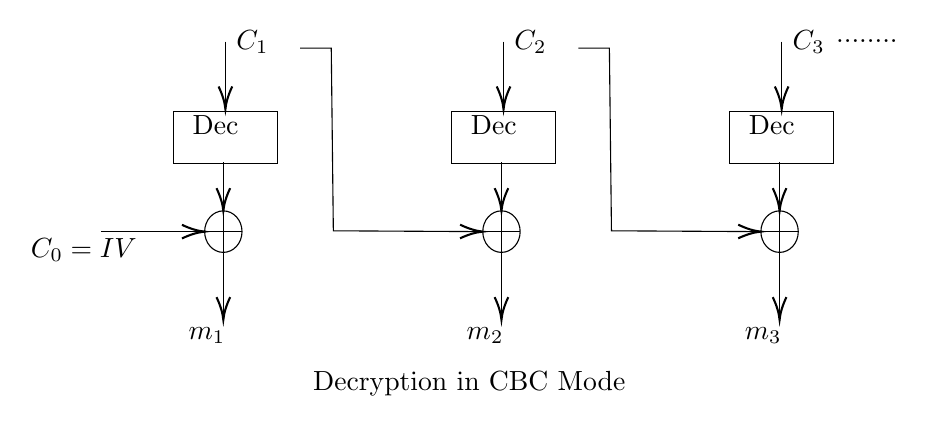
\begin{tikzpicture}[x=0.75pt,y=0.75pt,yscale=-1,xscale=1]
        \draw   (92,71) -- (142,71) -- (142,96) -- (92,96) -- cycle ; 
        \draw    (117,37.5) -- (117,68) ;
        \draw [shift={(117,70)}, rotate = 270] [color={rgb, 255:red, 0; green, 0; blue, 0 }  ][line width=0.75]    (10.93,-3.29) .. controls (6.95,-1.4) and (3.31,-0.3) .. (0,0) .. controls (3.31,0.3) and (6.95,1.4) .. (10.93,3.29)   ;
        \draw    (116,95.5) -- (116,117) ;
        \draw [shift={(116,119)}, rotate = 270] [color={rgb, 255:red, 0; green, 0; blue, 0 }  ][line width=0.75]    (10.93,-3.29) .. controls (6.95,-1.4) and (3.31,-0.3) .. (0,0) .. controls (3.31,0.3) and (6.95,1.4) .. (10.93,3.29)   ;
        \draw   (107,129) .. controls (107,123.48) and (111.03,119) .. (116,119) .. controls (120.97,119) and (125,123.48) .. (125,129) .. controls (125,134.52) and (120.97,139) .. (116,139) .. controls (111.03,139) and (107,134.52) .. (107,129) -- cycle ; \draw   (107,129) -- (125,129) ; \draw   (116,119) -- (116,139) ;
        \draw    (57,129) -- (105,129) ;
        \draw [shift={(107,129)}, rotate = 180] [color={rgb, 255:red, 0; green, 0; blue, 0 }  ][line width=0.75]    (10.93,-3.29) .. controls (6.95,-1.4) and (3.31,-0.3) .. (0,0) .. controls (3.31,0.3) and (6.95,1.4) .. (10.93,3.29)   ;
        \draw    (116,139) -- (116,169.5) ;
        \draw [shift={(116,171.5)}, rotate = 270] [color={rgb, 255:red, 0; green, 0; blue, 0 }  ][line width=0.75]    (10.93,-3.29) .. controls (6.95,-1.4) and (3.31,-0.3) .. (0,0) .. controls (3.31,0.3) and (6.95,1.4) .. (10.93,3.29)   ;
        \draw   (226,71) -- (276,71) -- (276,96) -- (226,96) -- cycle ;
        \draw    (251,37.5) -- (251,68) ;
        \draw [shift={(251,70)}, rotate = 270] [color={rgb, 255:red, 0; green, 0; blue, 0 }  ][line width=0.75]    (10.93,-3.29) .. controls (6.95,-1.4) and (3.31,-0.3) .. (0,0) .. controls (3.31,0.3) and (6.95,1.4) .. (10.93,3.29)   ;
        \draw    (250,95.5) -- (250,117) ;
        \draw [shift={(250,119)}, rotate = 270] [color={rgb, 255:red, 0; green, 0; blue, 0 }  ][line width=0.75]    (10.93,-3.29) .. controls (6.95,-1.4) and (3.31,-0.3) .. (0,0) .. controls (3.31,0.3) and (6.95,1.4) .. (10.93,3.29)   ;
        \draw   (241,129) .. controls (241,123.48) and (245.03,119) .. (250,119) .. controls (254.97,119) and (259,123.48) .. (259,129) .. controls (259,134.52) and (254.97,139) .. (250,139) .. controls (245.03,139) and (241,134.52) .. (241,129) -- cycle ; \draw   (241,129) -- (259,129) ; \draw   (250,119) -- (250,139) ;
        \draw    (250,139) -- (250,169.5) ;
        \draw [shift={(250,171.5)}, rotate = 270] [color={rgb, 255:red, 0; green, 0; blue, 0 }  ][line width=0.75]    (10.93,-3.29) .. controls (6.95,-1.4) and (3.31,-0.3) .. (0,0) .. controls (3.31,0.3) and (6.95,1.4) .. (10.93,3.29)   ;
        \draw   (360,71) -- (410,71) -- (410,96) -- (360,96) -- cycle ;
        \draw    (385,37.5) -- (385,68) ;
        \draw [shift={(385,70)}, rotate = 270] [color={rgb, 255:red, 0; green, 0; blue, 0 }  ][line width=0.75]    (10.93,-3.29) .. controls (6.95,-1.4) and (3.31,-0.3) .. (0,0) .. controls (3.31,0.3) and (6.95,1.4) .. (10.93,3.29)   ;
        \draw    (384,95.5) -- (384,117) ;
        \draw [shift={(384,119)}, rotate = 270] [color={rgb, 255:red, 0; green, 0; blue, 0 }  ][line width=0.75]    (10.93,-3.29) .. controls (6.95,-1.4) and (3.31,-0.3) .. (0,0) .. controls (3.31,0.3) and (6.95,1.4) .. (10.93,3.29)   ;
        \draw   (375,129) .. controls (375,123.48) and (379.03,119) .. (384,119) .. controls (388.97,119) and (393,123.48) .. (393,129) .. controls (393,134.52) and (388.97,139) .. (384,139) .. controls (379.03,139) and (375,134.52) .. (375,129) -- cycle ; \draw   (375,129) -- (393,129) ; \draw   (384,119) -- (384,139) ;
        \draw    (384,139) -- (384,169.5) ;
        \draw [shift={(384,171.5)}, rotate = 270] [color={rgb, 255:red, 0; green, 0; blue, 0 }  ][line width=0.75]    (10.93,-3.29) .. controls (6.95,-1.4) and (3.31,-0.3) .. (0,0) .. controls (3.31,0.3) and (6.95,1.4) .. (10.93,3.29)   ;
        \draw    (153,40.6) -- (168,40.6) -- (169,128.6) -- (239,128.99) ;
        \draw [shift={(241,129)}, rotate = 180.32] [color={rgb, 255:red, 0; green, 0; blue, 0 }  ][line width=0.75]    (10.93,-3.29) .. controls (6.95,-1.4) and (3.31,-0.3) .. (0,0) .. controls (3.31,0.3) and (6.95,1.4) .. (10.93,3.29)   ;
        \draw    (287,40.6) -- (302,40.6) -- (303,128.6) -- (373,128.99) ;
        \draw [shift={(375,129)}, rotate = 180.32] [color={rgb, 255:red, 0; green, 0; blue, 0 }  ][line width=0.75]    (10.93,-3.29) .. controls (6.95,-1.4) and (3.31,-0.3) .. (0,0) .. controls (3.31,0.3) and (6.95,1.4) .. (10.93,3.29)   ;
        
        \draw (100,72) node [anchor=north west][inner sep=0.75pt]   [align=left] {Dec};
        \draw (121,31) node [anchor=north west][inner sep=0.75pt]   [align=left] {$C_1$};
        \draw (22,131) node [anchor=north west][inner sep=0.75pt]   [align=left] {$C_0 = IV$};
        \draw (98,174) node [anchor=north west][inner sep=0.75pt]   [align=left] {$m_1$};
        \draw (234,72) node [anchor=north west][inner sep=0.75pt]   [align=left] {Dec};
        \draw (255,31) node [anchor=north west][inner sep=0.75pt]   [align=left] {$C_2$};
        \draw (232,174) node [anchor=north west][inner sep=0.75pt]   [align=left] {$m_2$};
        \draw (368,72) node [anchor=north west][inner sep=0.75pt]   [align=left] {Dec};
        \draw (389,31) node [anchor=north west][inner sep=0.75pt]   [align=left] {$C_3$};
        \draw (366,174) node [anchor=north west][inner sep=0.75pt]   [align=left] {$m_3$};
        \draw (410,35) node [anchor=north west][inner sep=0.75pt]   [align=left] {........};
        \draw (158,195) node [anchor=north west][inner sep=0.75pt]   [align=left] {Decryption in CBC Mode};

    \end{tikzpicture}
\end{center}


\section{Hash Function}
It is a mapping from one set to another set.\\
\begin{center}
    $h : A \rightarrow B$\\
    $h(X) = Y$
\end{center}
Every hash function has following properties:
\begin{enumerate}
    \item If X is altered to $X'$, then h($X'$) will be completely different from h(X).
    \item Given Y, it is practically infeasible to find X s.t. h(X) = Y.
    \item Given X and Y = h(X), it is practically infeasible to find $X'$ s.t. h(X) = h($X'$).
\end{enumerate}
Let us consider this scenario where Alice is encrypting some message using symmetric key and sending it to Bob. 
\begin{center}
    

\tikzset{every picture/.style={line width=0.75pt}} %set default line width to 0.75pt        

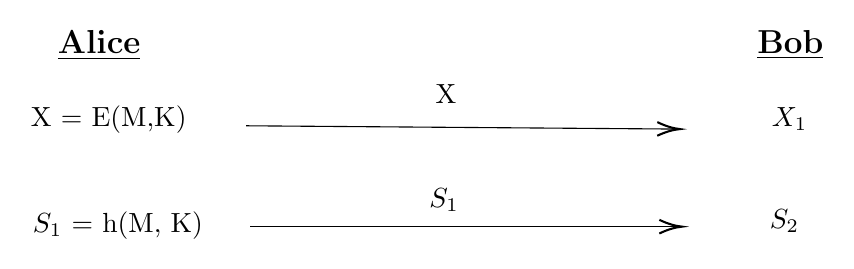
\begin{tikzpicture}[x=0.75pt,y=0.75pt,yscale=-1,xscale=1]
%uncomment if require: \path (0,300); %set diagram left start at 0, and has height of 300

%Straight Lines [id:da6936070700935975] 
\draw    (247,132) -- (454,133.58) ;
\draw [shift={(456,133.6)}, rotate = 180.44] [color={rgb, 255:red, 0; green, 0; blue, 0 }  ][line width=0.75]    (10.93,-3.29) .. controls (6.95,-1.4) and (3.31,-0.3) .. (0,0) .. controls (3.31,0.3) and (6.95,1.4) .. (10.93,3.29)   ;
%Straight Lines [id:da1977592175436449] 
\draw    (249,180.6) -- (455,180.6) ;
\draw [shift={(457,180.6)}, rotate = 180] [color={rgb, 255:red, 0; green, 0; blue, 0 }  ][line width=0.75]    (10.93,-3.29) .. controls (6.95,-1.4) and (3.31,-0.3) .. (0,0) .. controls (3.31,0.3) and (6.95,1.4) .. (10.93,3.29)   ;

% Text Node
\draw (155,85) node [anchor=north west][inner sep=0.75pt]   [align=left] {\textbf{{\large \underline{Alice}}}};
% Text Node
\draw (492,85) node [anchor=north west][inner sep=0.75pt]   [align=left] {\textbf{\underline{{\large Bob}}}};
% Text Node
\draw (142,121) node [anchor=north west][inner sep=0.75pt]   [align=left] {X = E(M,K)};
% Text Node
\draw (499,122) node [anchor=north west][inner sep=0.75pt]   [align=left] {$X_1$};
% Text Node
\draw (143,172) node [anchor=north west][inner sep=0.75pt]   [align=left] {$S_1$ = h(M, K)};
% Text Node
\draw (498,171) node [anchor=north west][inner sep=0.75pt]   [align=left] {$S_2$};
% Text Node
\draw (337,111) node [anchor=north west][inner sep=0.75pt]   [align=left] {X};
% Text Node
\draw (334,161) node [anchor=north west][inner sep=0.75pt]   [align=left] {$S_1$};


\end{tikzpicture}

\end{center}

Now, we want to verify that the message is coming from Alice and it has not been altered. Suppose if Bob receives the altered cipher text
$\tilde{X}$. Then on decryption using key K, Bob will not get the message M. So we need to ensure that the cipher text is coming from Alice and has not been altered. For that we use hash function. \\
\begin{center}
    If h($X_1$, K) = $S_2$, then Bob accepts $X_1$.
\end{center}
Since for hash function, if the input is changed even slightly, there is huge change in output. So if $X_1$ would have been altered even on a single bit, the output will not satisfy. Also, since we know input $X_1$ and the output of h(M, K) = $S_2$, still because of the properties of hash function, we still cannot determine message m and it is secure.
This is known as the Message Authentication Code. We are able to verify :
\begin{itemize}
    \item Whether X is altered during communication
    \item Whether $S_1$ is altered during communication
\end{itemize}

\subsection{Definition}
A hash family is a four tuple (P, S, K, H where the following conditions are satisfied.
\begin{enumerate}
    \item P is the set of all possible messages
    \item S is the set of all possible message digests or authentication tags(all output)
    \item K is the key space
    \item For each $K_1 \in k$, there is a hash function $h_{K_1}$ such that
    \begin{center}
        $h_{K_1} : P \rightarrow S$\\
        where $|P| \geq |S|$\\
        more interestingly $|P| \geq 2\times |S|$\\
    \end{center}
\end{enumerate}
\begin{center}
    

\tikzset{every picture/.style={line width=0.75pt}} %set default line width to 0.75pt        

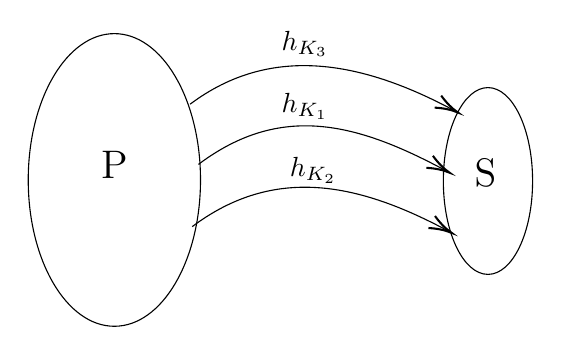
\begin{tikzpicture}[x=0.75pt,y=0.75pt,yscale=-1,xscale=1]
%uncomment if require: \path (0,300); %set diagram left start at 0, and has height of 300

%Shape: Ellipse [id:dp6385929644721748] 
\draw   (130.2,139.1) .. controls (130.2,100.16) and (148.78,68.6) .. (171.7,68.6) .. controls (194.62,68.6) and (213.2,100.16) .. (213.2,139.1) .. controls (213.2,178.04) and (194.62,209.6) .. (171.7,209.6) .. controls (148.78,209.6) and (130.2,178.04) .. (130.2,139.1) -- cycle ;
%Shape: Ellipse [id:dp35632658610404433] 
\draw   (330.2,139.6) .. controls (330.2,114.75) and (339.83,94.6) .. (351.7,94.6) .. controls (363.57,94.6) and (373.2,114.75) .. (373.2,139.6) .. controls (373.2,164.45) and (363.57,184.6) .. (351.7,184.6) .. controls (339.83,184.6) and (330.2,164.45) .. (330.2,139.6) -- cycle ;
%Curve Lines [id:da9831191387685083] 
\draw    (208.2,102.6) .. controls (247.8,72.9) and (292.3,82.4) .. (335.88,105.88) ;
\draw [shift={(337.2,106.6)}, rotate = 208.61] [color={rgb, 255:red, 0; green, 0; blue, 0 }  ][line width=0.75]    (10.93,-3.29) .. controls (6.95,-1.4) and (3.31,-0.3) .. (0,0) .. controls (3.31,0.3) and (6.95,1.4) .. (10.93,3.29)   ;
%Curve Lines [id:da7449905549695661] 
\draw    (212.2,131.6) .. controls (251.8,101.9) and (288.46,111.4) .. (331.88,134.88) ;
\draw [shift={(333.2,135.6)}, rotate = 208.61] [color={rgb, 255:red, 0; green, 0; blue, 0 }  ][line width=0.75]    (10.93,-3.29) .. controls (6.95,-1.4) and (3.31,-0.3) .. (0,0) .. controls (3.31,0.3) and (6.95,1.4) .. (10.93,3.29)   ;
%Curve Lines [id:da6241272700976574] 
\draw    (209.2,161.6) .. controls (248.8,131.9) and (289.38,140.42) .. (332.88,163.88) ;
\draw [shift={(334.2,164.6)}, rotate = 208.61] [color={rgb, 255:red, 0; green, 0; blue, 0 }  ][line width=0.75]    (10.93,-3.29) .. controls (6.95,-1.4) and (3.31,-0.3) .. (0,0) .. controls (3.31,0.3) and (6.95,1.4) .. (10.93,3.29)   ;

% Text Node
\draw (164,124) node [anchor=north west][inner sep=0.75pt]   [align=left] {{\Large P}};
% Text Node
\draw (344,128) node [anchor=north west][inner sep=0.75pt]   [align=left] {{\Large S}};
% Text Node
\draw (251,66) node [anchor=north west][inner sep=0.75pt]   [align=left] {$h_{K_3}$};
% Text Node
\draw (251,96) node [anchor=north west][inner sep=0.75pt]   [align=left] {$h_{K_1}$};
% Text Node
\draw (255,127) node [anchor=north west][inner sep=0.75pt]   [align=left] {$h_{K_2}$};


\end{tikzpicture}

Where H : set of all hash function
$h_{k_i}$ : hash function
\end{center}
\vspace{3mm}
\subsection{Types of Hash Function}
\begin{itemize}
    \item \textbf{Keyed Hash function : } In these hash functions, key is involved in the computation of hash value.
    \item \textbf{Unkeyed Hash function : } In these hash functions, key is not required to compute the hashed value.
\end{itemize}

\subsection{Problems}
\textbf{Problem 1:}\\
\begin{center}
    h : $ P \rightarrow S$
\end{center}
Given $y \in S$, find $x \in P$ such that h(x) = y. \\
\newline
This problem is known as the 'preimage finding problem'. For a hash function, h if you cannot find preimage in feasible time, then h is known as preimage resistant hash function. It is computationally difficult to find preimage for such functions.\\
\newline
\textbf{Problem 2:}\\
\begin{center}
    h : $ P \rightarrow S$
\end{center}
Given $x \in p$ and h(x), find $x' \in P$ such that $x' \neq x$ and $h(x') = h(x)$.\\
\newline
This problem is known as 'Second preimage finding problem'. If finding second preimage is computationally hard for h, then it is known as second preimage resistant hash function.\\
\newline
\textbf{Problem 3:}\\
\begin{center}
    h : $ P \rightarrow S$
\end{center}
Find x, $x' \in P$ such that $x \neq x'$ and $h(x) = h(x')$\\
\newline
This problem is known as collision finding problem. For a hash function h, if finding collision is computationally hard, then is known as collision resistant hash function.

\subsection{Ideal Hash Function}
Let $h : P \rightarrow S$ be a hash function.\\
h will be called ideal hash function if given $x \in P$ to find h(x) or either you have to apply h on x or you have to look into the table corresponding to h(hash table). If there are only these two ways, then it is ideal hash function.

\subsection{Pre image finding algorithm}
\begin{center}
    h : $X \rightarrow Y$
\end{center}
$|Y|=M$\\
Choose any $X_o \subseteq X$ such that $|X_o| = Q$\\
\begin{center}
\tikzset{every picture/.style={line width=0.75pt}} %set default line width to 0.75pt        

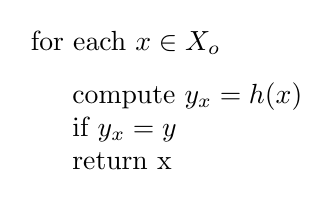
\begin{tikzpicture}[x=0.75pt,y=0.75pt,yscale=-1,xscale=1]
%uncomment if require: \path (0,300); %set diagram left start at 0, and has height of 300


% Text Node
\draw (114,67) node [anchor=north west][inner sep=0.75pt]   [align=left] {for each $x \in X_o$};
% Text Node
\draw (134,92) node [anchor=north west][inner sep=0.75pt]   [align=left] {compute $y_x = h(x)$
\\if $y_x = y$
\\ return x};


\end{tikzpicture}

\end{center}
The chance of getting pre-image depends on the selection of $X_o$. \\
\newline
Let us find the probability of finding pre-image using $X_o$\\
\begin{center}
    $X_o = \{x_1, x_2, \dots , x_Q \}$\\
    $E_i : event h(x_i) = y; 1 \leq i \leq Q$
\end{center}
h(x) can have M values, out of which only one will give success. So,
\begin{center}
    $Pr[E_i] = \frac{1}{M}$\\
    $Pr[{E_i}'] = 1- \frac{1}{M}$
\end{center}
Now we accumulate the probabilities of $E_1, E_2 \dots E_Q$
\begin{center}
    $Pr[E_1 \cup E_2 \cup E_3 \cup \dots \cup E_Q] = 1 - Pr[{E_1}' \cap {E_2}' \cap {E_3}' \cap \dots \cap {E_Q}']$\\
    \vspace{3mm}
    $Pr[E_1 \cup E_2 \cup E_3 \cup \dots \cup E_Q] = 1 - \prod_{i=1}^{Q} Pr[{E_i}']$\\
    \vspace{3mm}
    $Pr[E_1 \cup E_2 \cup E_3 \cup \dots \cup E_Q] = 1 - {(1-\frac{1}{M})}^Q$
\end{center}
Let us expand it now. 
\begin{center}
    $Pr[E_1 \cup E_2 \cup E_3 \cup \dots \cup E_Q] = 1 - [1-(\binom{Q}{1} \frac{1}{M} + \binom{Q}{2} \frac{1}{M^2} \dots]$\\
    \vspace{3mm}
    $Pr[E_1 \cup E_2 \cup E_3 \cup \dots \cup E_Q] \approx  1 - [1-(\binom{Q}{1} \frac{1}{M}]$\\
    \vspace{3mm}
    $Pr[E_1 \cup E_2 \cup E_3 \cup \dots \cup E_Q] \approx \frac{Q}{M}$
\end{center}
Therefore, 
\begin{center}
    Pr[ pre image finding ] = $\frac{Q}{M}$\\
    \vspace{3mm}
    Complexity(pre image finding) = O(M)
\end{center}
\end{document}